%!TEX root = ../report.tex

\chapter{Conclusions}
\label{chap:conclusions}
\section{Conclusions}
Main contribution of this thesis is hyperparameter optimization and comparative analysis for DenseNet two-channel, DenseNet-Siamese, and VGG-Siamese network (with Contrastive loss), for sonar patch matching problem.
Results obtained in this work are improvement over previous state-of-the-art result. Using DenseNet Two-Channel network average prediction accuracy obtained is 0.955 area under ROC curve (AUC). 
VGG-Siamese (with Contrastive loss function) and DenseNet-Siamese perform the prediction with an average 
AUC of 0.949 and 0.921 respectively. All these results are an improvement over the result of 0.894 AUC from Valdenegro-Toro \cite{stateoftheart}. By encoding an ensemble of DenseNet two-channel and DenseNet-Siamese 
models with respective highest AUC scores, prediction accuracy for the Ensemble obtained is 0.978 AUC, which is overall highest accuracy recorded during the scope of this thesis.
Here, DenseNet and VGG networks were used as branches of Siamese network, for feature extraction. Such application of those networks in sonar image-processing field is also a contribution of this work.

Most important lesson learned during this work is how to encode CNNs to do sonar image processing, without manually designing any features. Also, it is observed that acoustic vision is very challenging and quite different from normal 
optical vision. 

\section{Future work}
Main limitation of the hyperparameter optimization process presented in this work is that, manually doing hyperparameter optimization is a tedious process and needs some prior experience to be able to predefine 
the search spaces effectively. Another limitation of the manual grid search is that it might miss the best values if the grid is not very fine. To make search grid very fine, the total size of the search space increases a lot. 
This work \cite{bergstra2012random} points at the same limitation of grid search method, also suggests random search can yield better results than grid search.

\begin{figure}[ht]
\centering
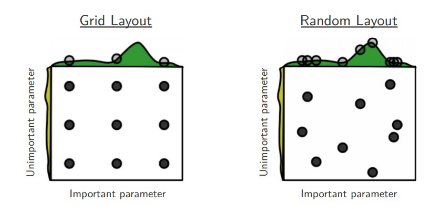
\includegraphics[height= 4cm]{images/densenet/random_search_over_grid_search}
\caption{Grid search vs random search from \cite{bergstra2012random}}
\label{fig:random_search_over_grid_search}
\end{figure}

Future work, for the thesis would be to perform hyperparameter optimization using an automatic algorithm, for example Bayesian Optimization \cite{snoek2012practical} or Sequential Model-based Algorithm Configuration (SMAC) \cite{hutter2011sequential} or 
Tree-structured Parzen Estimator (TPE) \cite{bergstra2011algorithms}. Automatic optimization process involves lesser human involvement and theoretically converges sooner.
FaceNet \cite{schroff2015facenet} with triplet loss function is one of the networks that is very interesting and applicable for the sonar patch matching problem. Such advance state-of-the art methods can be evalute
 %https://arimo.com/data-science/2016/bayesian-optimization-hyperparameter-tuning/
